\documentclass[10pt,a4paper]{report}
\usepackage[latin1]{inputenc}
\usepackage{amsmath}
\usepackage{amsfonts}
\usepackage{amssymb}
\usepackage{graphicx}
\usepackage{url}
\usepackage{listings}
\usepackage{xcolor}
\lstset{
numbers=left,
numberstyle=\small,
frame=signal,
framesep=4mm,
framexleftmargin=4mm,
backgroundcolor=\color{gray!10!white},
}
\begin{document}
\title{SDMengine manual\\{\small Version: 0.1}\\{\small For software version: 0.1}}
\author{}
\date{2014-12-9}
\maketitle
\chapter{Introduce SDMengine}
SDMengine is a software build for ecologist to study species distribution modelling, the designing mind of SDMengine different from other same function software like Biomod2, dismo or openmodeller. The most different is SDMengine have three import rule to guide design work:
\begin{itemize}
\item Configure better than programming
\item Do not repeat by yourself
\item Universal better than your private
\end{itemize}


\section{Configure better then programming}
The first import thing to guide design work is configure better than programming, for normal user of modelling build tools or software, their don't have some many knowledge about programming language, even a well trained professional programmer to read other people's code also take some time and sometimes it is not easy to understand what there to do with poor comment or document.

All this make read other people's code is unpleased or hard work for researcher no matter your have great programming knowledge or not. Unfortunately, most of current modelling software not design for end user, their designed for program, this kind of design have great flexible, user can do second development on this software to build a more user-oriented software. In real case, user always development their own-used only or this-project-only program. Such self-made program is very suit for their self or their project, but the code is always really hard read and reuse by other people who don't join this team or this project. To understand what the author really do will cost searcher a lot of work and it's a very hard and boring work.

Ours first rule "configure better than programming" is our striate to resolve the problem, by provide a wide usable configurable software: SDMengine. SDMengine is design to be widely usable, so many researcher can use it, and more import it's configure-oriented. that means we are not courage user to change the code while we courage user to change configure file (by hand-write or GUI-base programe assisted). By this method other researcher only need to read configure will know all the key information about the authors work.

\section{Do not repeat by yourself}
Do not repeat by your self, this is widely used rule for many thing, programmer develop software and distribution to user is want user not repate this work by themself, this is a very import way to improve efficiency. We use it as sencond rule because it's import to user and software developer like us.

\section{Universal better than your private}
SDMengine not only a tools to build modelling but also a tools to analysis result. We courage user distribution their analysis script to other user so everyone will benifit from this. And we don't courage user develop a function that already exists if their function work better. Because already exists analysis script will test by many user, code will check by many programmer so this will make script have high quietly. This make user to analysis better and easily.

\section{Implement of SDMengine}
User should notice that SDMengine is not a signal software but also protocol standard. SDMengine software just a implement of SDMengine protocol. Simllar things is like USB protocol and USB disk, any USB disk implemented USB protocal can communicate with other USB device (for example, personal computer). For PC, different band of USB disk are excately same when using them.
\subsection{Design of Implement}
SDMengine protocol is not design for some specific language or platform (MAC, UNIX, Linux are suitable, for the reason that windows not suit for high-performance-compute, windows are not courage but still usable). Modelling technolgy change with times and so the modelling library and platform. For this reason SDMengine not depend on any language. The implement of SDMengine will read same input data and configure and output exactly same not matter which language the implement used. To meet so demand, input data, configure and output data are universal format.
\subsection{Current Implement}
As first implement of SDMengine, we use R language as program language for R language was widely used in species distribuiton modelling domain. 
\section{Structure of SDMengine}
\subsection{Overall view of structure}
SDMengine are base on filesystem. First thing to begin use SDMengine is build workshop directory. Don't worry, We proved a tool to do this job.
\begin{quote}
build\_workshop.R
\end{quote}
By default use without params, tool will build a directory under curren work directory named "workshop". the struct of this directory is shown in Figure.\ref{fig:workshop_structure}:



There are five directory:
\begin{itemize}
\item species
\item environment
\item configure
\item result
\item database
\end{itemize}

\subsubsection{Directory of species}
Directory of species are species data, each species data are directory contained "presence" map and "absence" map. if species name contain more then two words (it always contain at lest two words) please use - as hyphen, not suggest use \_ or blank char "\ " (e.g. virutal-species).

\begin{figure}[h]
\centering
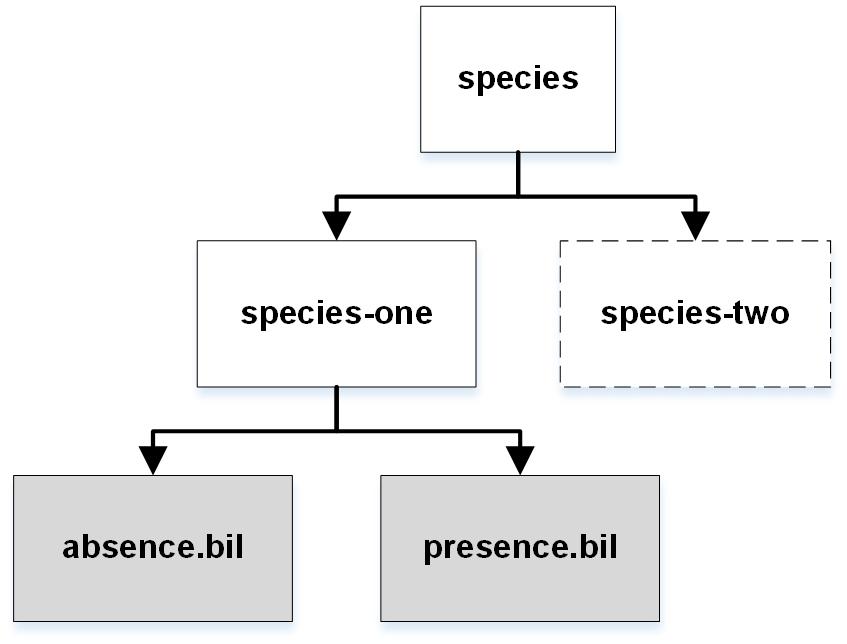
\includegraphics[angle=0,width=0.55\linewidth]{species_directory.jpg}
\caption[workshop]{Structure of species directory}
\label{fig:workshop_structure}
\end{figure}


\subsubsection{Directory of environment}
Directory of environment set, notice that by default there use base as current environment data set. Inner environment data file better don't use some special char. that may cause something unpredectable.

\begin{figure}[h]
\centering
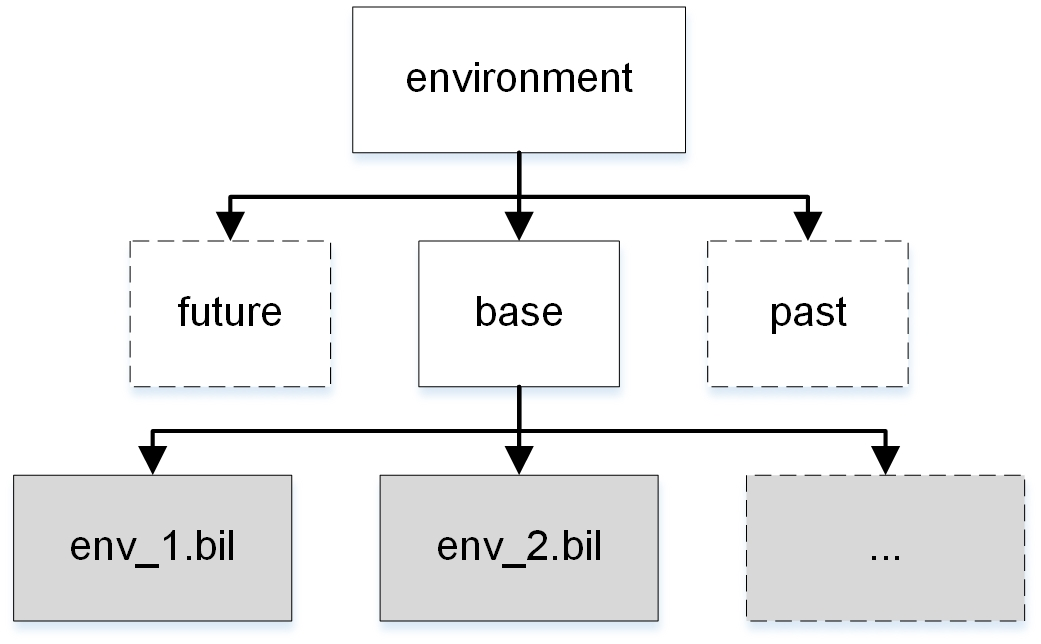
\includegraphics[angle=0,width=0.55\linewidth]{environment_directory.jpg}
\caption[workshop]{Structure of species directory}
\label{fig:workshop_structure}
\end{figure}

\subsubsection{Directory of configure}
This Directory currently contain only one file named "configure.yaml". This file was in "YAML" format, we choose "YAML" as format becasue it's very user-friendly, syntax is very easy to read and write.

\begin{figure}[h]
\centering
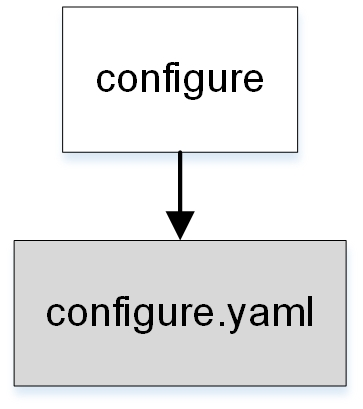
\includegraphics[angle=0,width=0.2\linewidth]{configure.jpg}
\caption[workshop]{Structure of species directory}
\label{fig:workshop_structure}
\end{figure}



\subsubsection{Directory of result}
All SDMengine map will output to this directory, directory was create automaticly. Subdirectory sequence was

\begin{figure}[h]
\centering
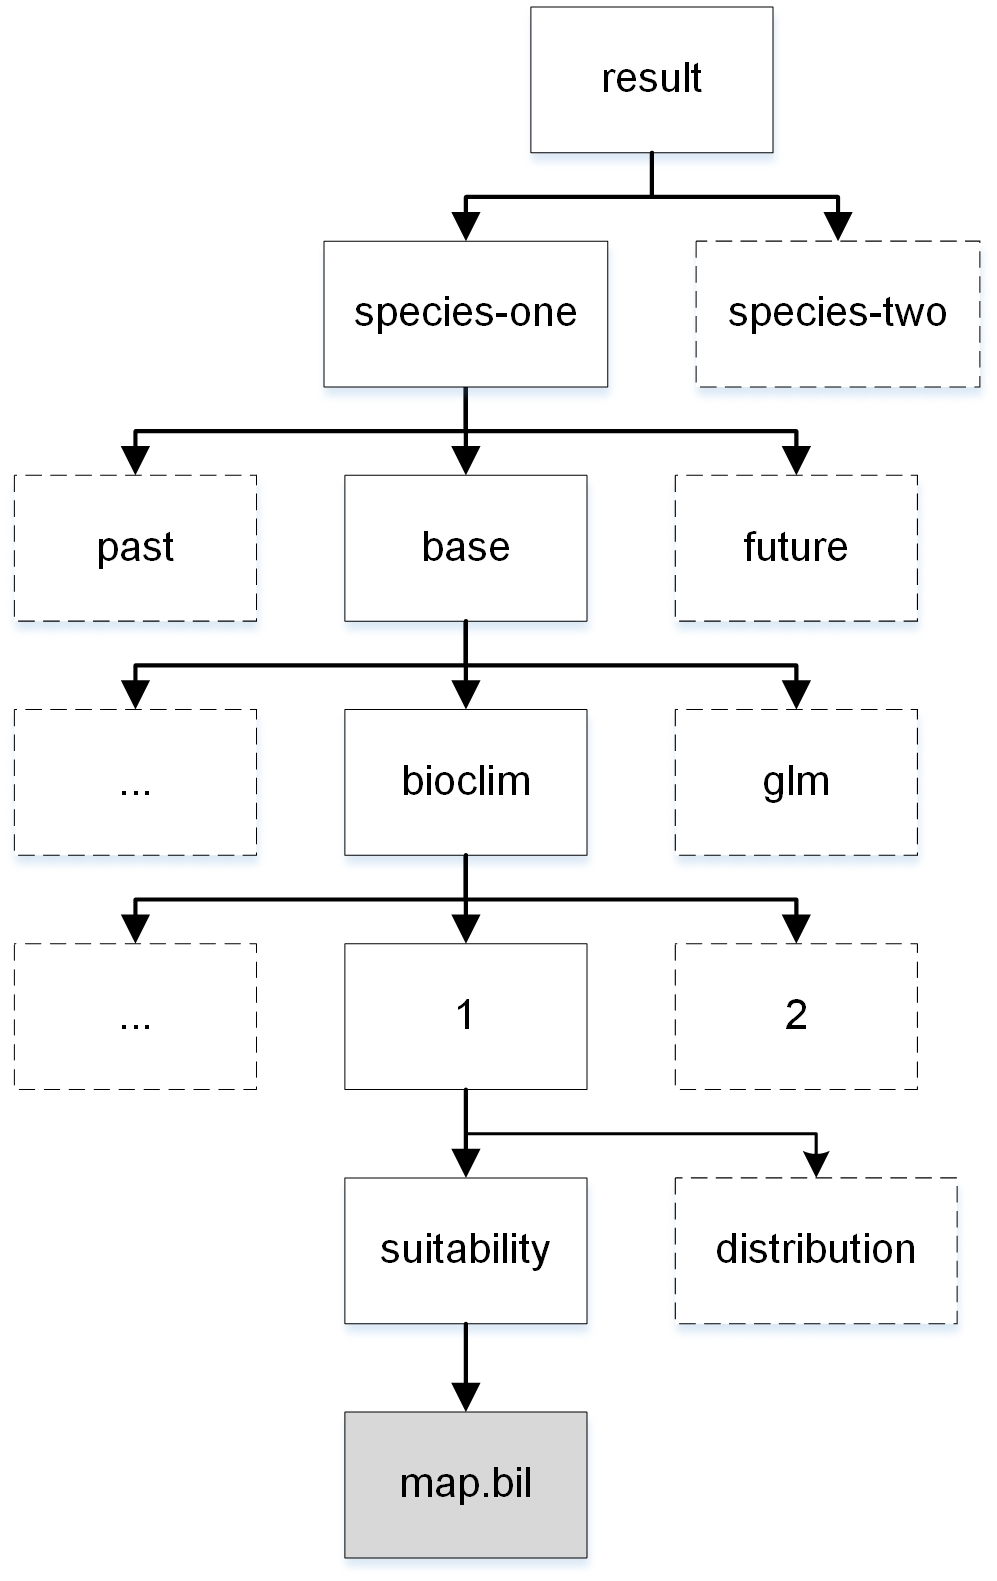
\includegraphics[angle=0,width=0.55\linewidth]{result-directory.jpg}
\caption[workshop]{Structure of species directory}
\label{fig:workshop_structure}
\end{figure}

\begin{enumerate}
\item species
\item runtimes
\item method
\item environment
\item suitability and distributon
\end{enumerate}

For example see Figure.\ref{fig:workshop_structure}.

\subsubsection{Directory of database}
All critenrion will store in a database (SQLite database). This file named "meta.db".

\section{Usage of SDMengine}
\subsection{Prepare of data}
Before start run SDMengine, some data need to be prepare. 
\begin{itemize}
\item Species distribution data split to absence map and presence map
\item Collect environment data set that relative to species
\item Write or change configure file
\end{itemize}

\subsubsection{Species distribution}
Your species disribution data need to split to two map (raster map only): 1) absence map named "absence.*", 2) presence map named "presence.*". "*" presencent GDAL geography format.

\subsubsection{Environment data set}
Environment file should have same cell size with species map and at last cover species data extend. if user predict climate change or some time shift things may have two environment directory, the environment of species map have a static name "base", if you predict future climate change infect on species distribution, you may set a subdirectory name "future" (other directory name is OK, but name better have some meaning like "2050s"), see Figure.\ref{fig:workshop_structure}. for demo.

\subsubsection{Configure}
Configure file are write in "YAML" format. Default setting already have been written.

\subsection{Tips on Raster Formats}
As well as many other open source software we use GDAL (Geospatial Data Abstraction Library; http://www.gdal.org/) as backend library to handle geospatial file.

GDAL support many format, for more detail see web page(http://www.gdal.org/formats\_list.html). We suggest user use only a few format below:

\begin{tabular}{|c|c|c|c|}
\hline  rank & Long format name & Code & append name \\ 
\hline  1 & ESRI .hdr Labelled & EHdr & main file: *.bil \\ 
\hline  2 & ENVI .hdr Labelled Raster & ENVI & main file: *.bil \\ 
\hline  3 & FARSITE v.4 LCP Format & LCP &  \\ 
\hline  4 & Vexcel MFF & MFF &  \\ 
\hline  5 & Vexcel MFF2 & MFF2 (HKV) &  \\ 
\hline  6 & PCI Geomatics Database File & PCIDSK &  \\ 
\hline  7 & Idrisi Raster & RST &  \\ 
\hline 
\end{tabular}

Usually we suggest user use rank 1 format because this is very widely used and this format was use by WorldClim (http://worldclim.org/) which climate data was widely use in SDM. Using other format will need user translate the format.

Current version of SDMengine default use "ESRI .hdr Labelled" as raster format for input and output. so currently user only can use this format.

\subsection{Run SDMengine}
When done with prepare process. Now can run SDMengine main tools. Current implement of SDMengine are write in R language, so the high-preformace we choose mutl-process. Defalut will open 4 process to run modelling.

\section{Configure}
SDMengine using YAML (YAML Ain't Markup Language) as configure file format. YAML is a human friendly data serialization standard for all programming languages. We recommand use write configure in YAML 1.2 (3rd Edition) syntax (\url{http://www.yaml.org/spec/1.2/spec.html}).

Here we document general usage of configure.yaml.

\lstinputlisting{configure.yaml}

\subsection{"engine"}
First line "engine" specification the basement-engine which do the real modelling work. currently only "dismo" version implement is done. So let it be "dismo" always.

\subsection{"species\_name"}
Second line "species\_name" specification the species you want to modelling, SDMengine allow you modelling all the species that contained in species directory or part of them. If that set to be "true", meanings all the species in the species directory will be modelling. if you want modelling only part of them. Just list them like this.

\begin{lstlisting}
species_name:
- species_one
- species_two
\end{lstlisting}

Should notice that even modelling only one species, you still write like a list. 

\begin{lstlisting}
species_name:
- only_one_species
\end{lstlisting}

Below is not support.

\begin{lstlisting}
species_name: only_one_species
\end{lstlisting}

\subsection{"run\_times"}
Third Line "run\_times", cause of random select absence point into modelling, SDM always repeat certain times to remove random affection. Item "run\_time" is used to indicated repeat times.

\subsection{"background\_point"}
specification the backgroud\_point that modelling will take from backgroud. if it set to 'null' it will using system default value, currently is 500.

\subsection{"presence\_point"}
specification the presence\_point. if it set to 'null' it will take all presence point into modelling, if you set to a number, system will take as maxnium as it can to close this number, that means if you presence point less than this number, system will take all the point.

\subsection{"predict"}
SDMengine sometine used to modelling some shifting case (space shifting or space shifting). You can predict other environment set. if you set predict to 'true' that means you predict all the environment set (scene). If you only want predict some of them. Just like "species\_name".


\begin{lstlisting}
predict:
- environment_set_one
- environment_set_two
\end{lstlisting}

and this is good:

\begin{lstlisting}
species_name:
- only_one_environment_set
\end{lstlisting}

Below is not support.

\begin{lstlisting}
species_name: only_one_environment_set
\end{lstlisting}

\subsection{"environment\_layer"}
if you want use only part of environment set layer, you can use this to setup. set them to 'true' if you want using all environment layer.

\subsection{"algorithms"}
list the algorithms you want to use. that realy depends on implement, so check the document on implement. And 'true' is not accept here.

\section{Analysis result}
SDMengine can co-work with an analysis tools named "SDManalysis". SDManalysis only work with SDMengine but split with SDMengine. Of course user can write private script to analysis but we suggest user use SDManalysis that can benifit some advantage of SDMengine and SDManalysis community.  




\end{document}